% 模块层次结构图
% 使用方法: 在主文档中 % 模块层次结构图
% 使用方法: 在主文档中 % 模块层次结构图
% 使用方法: 在主文档中 % 模块层次结构图
% 使用方法: 在主文档中 \input{figures/module_hierarchy.tex}
% 字体: 中文使用宋体（继承文档设置），英文使用 Times New Roman（newtxtext）

\begin{tikzpicture}[
    every node/.append style={font=\rmfamily},  % 确保使用衬线字体（Times/宋体）
    level 1/.style={sibling distance=3.8cm, level distance=1.5cm},
    level 2/.style={sibling distance=1.8cm, level distance=1.3cm},
    level 3/.style={sibling distance=1.5cm, level distance=1.2cm},
    module/.style={draw, thick, rounded corners=2pt, fill=blue!10, minimum width=1.8cm, minimum height=0.6cm, align=center, font=\tiny},
    submodule/.style={draw, rounded corners=2pt, fill=green!10, minimum width=1.4cm, minimum height=0.5cm, align=center, font=\tiny},
    leaf/.style={draw, rounded corners=2pt, fill=yellow!10, minimum width=1.2cm, minimum height=0.4cm, align=center, font=\tiny},
    edge from parent/.style={draw, thick, ->,>=stealth},
]

\node[module, minimum width=3cm, fill=blue!20] (top) {schur\_kernel\_top}
    child {node[module] {axi\_lite\_slave}
        child {node[submodule] {register\_file}}
    }
    child {node[module] {axi\_mm\_master}
        child {node[submodule] {read\_engine}}
        child {node[submodule] {write\_engine}}
    }
    child {node[module] {main\_fsm}}
    child {node[module] {input\_buffer}
        child {node[leaf] {state\_param\_buf}}
        child {node[leaf] {sob\_buf}}
        child {node[leaf] {pts\_pw\_buf}}
        child {node[leaf] {feature\_uv\_buf}}
    }
    child {node[module] {coord\_transform\_unit}
        child {node[leaf] {quat\_mult}}
        child {node[leaf] {quat\_conj}}
        child {node[leaf] {quat\_rotate}}
        child {node[leaf] {quat\_to\_rotmat}}
        child {node[leaf] {mat3x3\_mult}}
    }
    child {node[module] {jacobian\_unit}
        child {node[leaf] {residual\_calc}}
        child {node[leaf] {huber\_scale}}
        child {node[leaf] {dr\_dpc\_calc}}
        child {node[leaf] {dpc\_dpos\_calc}}
        child {node[leaf] {jx\_calc}}
        child {node[leaf] {jf\_calc}}
    }
    child {node[module] {hessian\_accum\_unit}
        child {node[leaf] {jxT\_jx\_accum}}
        child {node[leaf] {jfT\_jf\_accum}}
        child {node[leaf] {jxT\_jf\_store}}
        child {node[leaf] {jxT\_r\_accum}}
        child {node[leaf] {jfT\_r\_accum}}
    }
    child {node[module] {intermediate\_buffer}
        child {node[leaf] {tmp\_amtx\_buf}}
        child {node[leaf] {tmp\_bvct\_buf}}
        child {node[leaf] {tmp\_v\_buf}}
        child {node[leaf] {tmp\_gv\_buf}}
        child {node[leaf] {tmp\_w\_buf}}
    }
    child {node[module] {schur\_elim\_unit}
        child {node[leaf] {mat3x3\_inv}}
        child {node[leaf] {w\_vinv\_mult}}
        child {node[leaf] {wvinv\_wT\_mult}}
        child {node[leaf] {wvinv\_g\_mult}}
        child {node[leaf] {a\_update}}
    }
    child {node[module] {output\_buffer}}
    child {node[module] {fp64\_unit}
        child {node[leaf] {fp64\_add[N]}}
        child {node[leaf] {fp64\_mul[M]}}
        child {node[leaf] {fp64\_div}}
        child {node[leaf] {fp64\_sqrt}}
    };

\end{tikzpicture}

% 字体: 中文使用宋体（继承文档设置），英文使用 Times New Roman（newtxtext）

\begin{tikzpicture}[
    every node/.append style={font=\rmfamily},  % 确保使用衬线字体（Times/宋体）
    level 1/.style={sibling distance=3.8cm, level distance=1.5cm},
    level 2/.style={sibling distance=1.8cm, level distance=1.3cm},
    level 3/.style={sibling distance=1.5cm, level distance=1.2cm},
    module/.style={draw, thick, rounded corners=2pt, fill=blue!10, minimum width=1.8cm, minimum height=0.6cm, align=center, font=\tiny},
    submodule/.style={draw, rounded corners=2pt, fill=green!10, minimum width=1.4cm, minimum height=0.5cm, align=center, font=\tiny},
    leaf/.style={draw, rounded corners=2pt, fill=yellow!10, minimum width=1.2cm, minimum height=0.4cm, align=center, font=\tiny},
    edge from parent/.style={draw, thick, ->,>=stealth},
]

\node[module, minimum width=3cm, fill=blue!20] (top) {schur\_kernel\_top}
    child {node[module] {axi\_lite\_slave}
        child {node[submodule] {register\_file}}
    }
    child {node[module] {axi\_mm\_master}
        child {node[submodule] {read\_engine}}
        child {node[submodule] {write\_engine}}
    }
    child {node[module] {main\_fsm}}
    child {node[module] {input\_buffer}
        child {node[leaf] {state\_param\_buf}}
        child {node[leaf] {sob\_buf}}
        child {node[leaf] {pts\_pw\_buf}}
        child {node[leaf] {feature\_uv\_buf}}
    }
    child {node[module] {coord\_transform\_unit}
        child {node[leaf] {quat\_mult}}
        child {node[leaf] {quat\_conj}}
        child {node[leaf] {quat\_rotate}}
        child {node[leaf] {quat\_to\_rotmat}}
        child {node[leaf] {mat3x3\_mult}}
    }
    child {node[module] {jacobian\_unit}
        child {node[leaf] {residual\_calc}}
        child {node[leaf] {huber\_scale}}
        child {node[leaf] {dr\_dpc\_calc}}
        child {node[leaf] {dpc\_dpos\_calc}}
        child {node[leaf] {jx\_calc}}
        child {node[leaf] {jf\_calc}}
    }
    child {node[module] {hessian\_accum\_unit}
        child {node[leaf] {jxT\_jx\_accum}}
        child {node[leaf] {jfT\_jf\_accum}}
        child {node[leaf] {jxT\_jf\_store}}
        child {node[leaf] {jxT\_r\_accum}}
        child {node[leaf] {jfT\_r\_accum}}
    }
    child {node[module] {intermediate\_buffer}
        child {node[leaf] {tmp\_amtx\_buf}}
        child {node[leaf] {tmp\_bvct\_buf}}
        child {node[leaf] {tmp\_v\_buf}}
        child {node[leaf] {tmp\_gv\_buf}}
        child {node[leaf] {tmp\_w\_buf}}
    }
    child {node[module] {schur\_elim\_unit}
        child {node[leaf] {mat3x3\_inv}}
        child {node[leaf] {w\_vinv\_mult}}
        child {node[leaf] {wvinv\_wT\_mult}}
        child {node[leaf] {wvinv\_g\_mult}}
        child {node[leaf] {a\_update}}
    }
    child {node[module] {output\_buffer}}
    child {node[module] {fp64\_unit}
        child {node[leaf] {fp64\_add[N]}}
        child {node[leaf] {fp64\_mul[M]}}
        child {node[leaf] {fp64\_div}}
        child {node[leaf] {fp64\_sqrt}}
    };

\end{tikzpicture}

% 字体: 中文使用宋体（继承文档设置），英文使用 Times New Roman（newtxtext）

\begin{tikzpicture}[
    every node/.append style={font=\rmfamily},  % 确保使用衬线字体（Times/宋体）
    level 1/.style={sibling distance=3.8cm, level distance=1.5cm},
    level 2/.style={sibling distance=1.8cm, level distance=1.3cm},
    level 3/.style={sibling distance=1.5cm, level distance=1.2cm},
    module/.style={draw, thick, rounded corners=2pt, fill=blue!10, minimum width=1.8cm, minimum height=0.6cm, align=center, font=\tiny},
    submodule/.style={draw, rounded corners=2pt, fill=green!10, minimum width=1.4cm, minimum height=0.5cm, align=center, font=\tiny},
    leaf/.style={draw, rounded corners=2pt, fill=yellow!10, minimum width=1.2cm, minimum height=0.4cm, align=center, font=\tiny},
    edge from parent/.style={draw, thick, ->,>=stealth},
]

\node[module, minimum width=3cm, fill=blue!20] (top) {schur\_kernel\_top}
    child {node[module] {axi\_lite\_slave}
        child {node[submodule] {register\_file}}
    }
    child {node[module] {axi\_mm\_master}
        child {node[submodule] {read\_engine}}
        child {node[submodule] {write\_engine}}
    }
    child {node[module] {main\_fsm}}
    child {node[module] {input\_buffer}
        child {node[leaf] {state\_param\_buf}}
        child {node[leaf] {sob\_buf}}
        child {node[leaf] {pts\_pw\_buf}}
        child {node[leaf] {feature\_uv\_buf}}
    }
    child {node[module] {coord\_transform\_unit}
        child {node[leaf] {quat\_mult}}
        child {node[leaf] {quat\_conj}}
        child {node[leaf] {quat\_rotate}}
        child {node[leaf] {quat\_to\_rotmat}}
        child {node[leaf] {mat3x3\_mult}}
    }
    child {node[module] {jacobian\_unit}
        child {node[leaf] {residual\_calc}}
        child {node[leaf] {huber\_scale}}
        child {node[leaf] {dr\_dpc\_calc}}
        child {node[leaf] {dpc\_dpos\_calc}}
        child {node[leaf] {jx\_calc}}
        child {node[leaf] {jf\_calc}}
    }
    child {node[module] {hessian\_accum\_unit}
        child {node[leaf] {jxT\_jx\_accum}}
        child {node[leaf] {jfT\_jf\_accum}}
        child {node[leaf] {jxT\_jf\_store}}
        child {node[leaf] {jxT\_r\_accum}}
        child {node[leaf] {jfT\_r\_accum}}
    }
    child {node[module] {intermediate\_buffer}
        child {node[leaf] {tmp\_amtx\_buf}}
        child {node[leaf] {tmp\_bvct\_buf}}
        child {node[leaf] {tmp\_v\_buf}}
        child {node[leaf] {tmp\_gv\_buf}}
        child {node[leaf] {tmp\_w\_buf}}
    }
    child {node[module] {schur\_elim\_unit}
        child {node[leaf] {mat3x3\_inv}}
        child {node[leaf] {w\_vinv\_mult}}
        child {node[leaf] {wvinv\_wT\_mult}}
        child {node[leaf] {wvinv\_g\_mult}}
        child {node[leaf] {a\_update}}
    }
    child {node[module] {output\_buffer}}
    child {node[module] {fp64\_unit}
        child {node[leaf] {fp64\_add[N]}}
        child {node[leaf] {fp64\_mul[M]}}
        child {node[leaf] {fp64\_div}}
        child {node[leaf] {fp64\_sqrt}}
    };

\end{tikzpicture}

% 字体: 中文使用宋体（继承文档设置），英文使用 Times New Roman（newtxtext）

\begin{tikzpicture}[
    every node/.append style={font=\rmfamily},  % 确保使用衬线字体（Times/宋体）
    level 1/.style={sibling distance=3.8cm, level distance=1.5cm},
    level 2/.style={sibling distance=1.8cm, level distance=1.3cm},
    level 3/.style={sibling distance=1.5cm, level distance=1.2cm},
    module/.style={draw, thick, rounded corners=2pt, fill=blue!10, minimum width=1.8cm, minimum height=0.6cm, align=center, font=\tiny},
    submodule/.style={draw, rounded corners=2pt, fill=green!10, minimum width=1.4cm, minimum height=0.5cm, align=center, font=\tiny},
    leaf/.style={draw, rounded corners=2pt, fill=yellow!10, minimum width=1.2cm, minimum height=0.4cm, align=center, font=\tiny},
    edge from parent/.style={draw, thick, ->,>=stealth},
]

\node[module, minimum width=3cm, fill=blue!20] (top) {schur\_kernel\_top}
    child {node[module] {axi\_lite\_slave}
        child {node[submodule] {register\_file}}
    }
    child {node[module] {axi\_mm\_master}
        child {node[submodule] {read\_engine}}
        child {node[submodule] {write\_engine}}
    }
    child {node[module] {main\_fsm}}
    child {node[module] {input\_buffer}
        child {node[leaf] {state\_param\_buf}}
        child {node[leaf] {sob\_buf}}
        child {node[leaf] {pts\_pw\_buf}}
        child {node[leaf] {feature\_uv\_buf}}
    }
    child {node[module] {coord\_transform\_unit}
        child {node[leaf] {quat\_mult}}
        child {node[leaf] {quat\_conj}}
        child {node[leaf] {quat\_rotate}}
        child {node[leaf] {quat\_to\_rotmat}}
        child {node[leaf] {mat3x3\_mult}}
    }
    child {node[module] {jacobian\_unit}
        child {node[leaf] {residual\_calc}}
        child {node[leaf] {huber\_scale}}
        child {node[leaf] {dr\_dpc\_calc}}
        child {node[leaf] {dpc\_dpos\_calc}}
        child {node[leaf] {jx\_calc}}
        child {node[leaf] {jf\_calc}}
    }
    child {node[module] {hessian\_accum\_unit}
        child {node[leaf] {jxT\_jx\_accum}}
        child {node[leaf] {jfT\_jf\_accum}}
        child {node[leaf] {jxT\_jf\_store}}
        child {node[leaf] {jxT\_r\_accum}}
        child {node[leaf] {jfT\_r\_accum}}
    }
    child {node[module] {intermediate\_buffer}
        child {node[leaf] {tmp\_amtx\_buf}}
        child {node[leaf] {tmp\_bvct\_buf}}
        child {node[leaf] {tmp\_v\_buf}}
        child {node[leaf] {tmp\_gv\_buf}}
        child {node[leaf] {tmp\_w\_buf}}
    }
    child {node[module] {schur\_elim\_unit}
        child {node[leaf] {mat3x3\_inv}}
        child {node[leaf] {w\_vinv\_mult}}
        child {node[leaf] {wvinv\_wT\_mult}}
        child {node[leaf] {wvinv\_g\_mult}}
        child {node[leaf] {a\_update}}
    }
    child {node[module] {output\_buffer}}
    child {node[module] {fp64\_unit}
        child {node[leaf] {fp64\_add[N]}}
        child {node[leaf] {fp64\_mul[M]}}
        child {node[leaf] {fp64\_div}}
        child {node[leaf] {fp64\_sqrt}}
    };

\end{tikzpicture}
